%TC: macro \marginfootnote [other]
%TC: envir SCfigure [] other
%TC: macrocount beginSCfigure [figure]
\documentclass[11pt,twoside]{report}
\usepackage{preamble}
\setcounter{chapter}{2}
\graphicspath{{../img/}}
\def\includebibliography{}

\externaldocument{introduction}
\externaldocument{background}
\externaldocument{morphometric-framework}
\externaldocument{morphometric-applications}
\externaldocument{resummation}
\externaldocument{aerosols}

\begin{document}
\chapter{Supercooled liquids and glasses}
\epigraph{Truly, he thought, the way of enlightenment is like unto half a mile of broken glass.}{Terry Pratchett, \emph{Mort}, (1987).}
\label{chapter:glass}

In the introduction we established the supercooled liquid in hard spheres as the extension of the stable liquid above the freezing density, where it is metastable to the crystal phase.
To provide proper context we will discuss supercooled liquids more generally here, including thermal systems where temperature is the more natural control parameter.
As such, we will be considering the effect of decreasing temperature on the supercooled liquid.

%\hl{This chapter is more of a conventional literature review.}

%% \subsection{Mean-field picture}
%% The infinite dimensional limit $d \to \infty$.

%% \subsection{Random first-order transition theory}
%% Perturbation from mean-field in $1/d$.

%% \subsection{Alternative pictures in physical dimensions}
%% For $d \le 3$
%% \subsubsection{Frustration-limited domain theory}
%% \subsubsection{Dynamical theories}

%% \subsection{Old intro stuff}

%% It is widely reported that glass is actually liquid, and as evidence of this the thickness of old windows at the bottom is pointed to.
%% This is actually a matter of some dispute, but contains a grain of truth.
%% Pre-modern methods of creating window glass involved spinning molten glass on magma to flatten it out.
%% Centrifugal forces caused the glass to be thicker on the outer disc, so panes of glass would always be heavier in one direction%
%% \marginfootnote{And personally, if I were setting an uneven pane of glass I would place the thicker and heavier part at the bottom.}.

%% To a soft matter physicist glass is a broader term, referring to a wide class of materials while the window glass of common parlance is referred to by its chemical name \emph{silicate}.
%% This class of materials share many features of being disordered etc \cite{?} although in some sense they are connected by what they do \emph{not} do: which is flow on human timescales.
%% When I refer to `glass' I will be using it in this broad technical sense of a state of matter.
%% Some examples besides silicate:
%% \begin{itemize}
%% \item Most of the ice in the universe exists in an amorphous state in comets \cite{?}
%% \item Ceramics
%% \item Plastics: amorphous polymers
%% \end{itemize}
%% Of more abstract nature which could be called glassy though they are not materials
%% \begin{itemize}
%% \item Gels: super glasses, liquid like bit plus a network/backbone which has glassy dynamics
%% \item Neural networks
%% \item Non-deterministic polynomial time (NP) problems
%% \end{itemize}
%% We will not be directly addressing the latter type of more abstract problems which could be considered glasses, although they are arguably related due to a similar underlying disorder.
%% We will be focusing on only the most rudimentary of glassy phenomenology: the dynamical arrest of liquids at high densities/low temperatures when crystallisation is avoided.
%% Especially as it manifests in hard spheres, which as discussed is the reference system of choice for simple liquids.

%% Personally, the observation that got me interested in the field is the entropy argument.
%% If one compares the difference between the entropy of the crystal and the glass, and extrapolates wildly one expects there to be a point where the glass has a lower entropy than the crystal.
%% This is not very meaningful by itself, as we have already established by discussing the crystal vibrational entropy can be quite subtle so it is possible for the liquid to have a lower vibrational entropy.
%% However, if one corrects this with more modern techniques to measure just the entropy corresponding to non-trivial motion we see that there is a point where the configurational (i.e.\ not purely vibrational) entropy vanishes: this would imply the system is frozen in a single configuration.
%% Such a point would define a transition to a genuine thermodynamic phase, an ideal glass.

%% Hard glasses: high elastic constants.
%% Colloidal suspensions: soft matter version, small elastic constants.
%% Same phenomenology though.
%% What is a glass?
%% Frozen in a (apparently) disordered state.
%% All sorts of glasses, structural, spin, orientational, electron, vortex.
%% Glasses formed by liquids, colloidal suspensions and polymers: traditional structural glasses.
%% Solid: doesn't flow on observational time, resists small/infinitesimal shear (acts like solid).
%% Amorphous, apparently amorphous: no periodic arrangement like in crystal.
%% Homogeneous makes useful for technology: useful for e.g.\ optical properties.

%First, we describe the phenomenology of supercooled liquids before delving into the specific theories to explain them.

\section{Properties of the supercooled liquid}
\label{sec:glass-phenomenology}

We will start by exploring the ways in which supercooled liquids are the \emph{same} as regular liquids, expanding in more detail on ideas discussed in the introduction.
Then we will move onto the ways in which they \emph{differ} from ordinary liquids, notably in their dynamical properties and their structure at the many-body level.

\begin{SCfigure}
  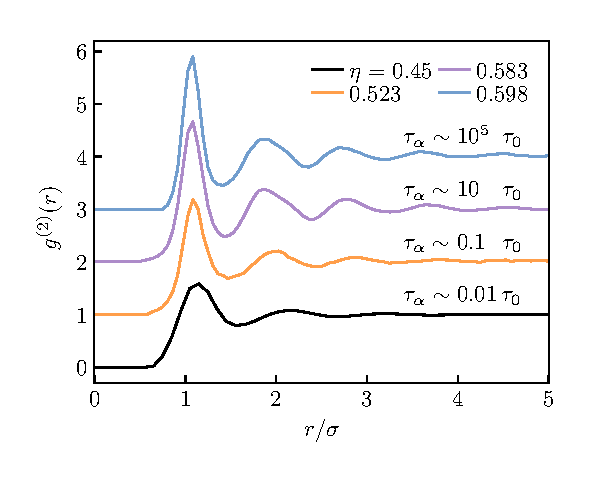
\includegraphics[width=0.9\linewidth,outer]{g2-evolution}
  %\missingfigure[figwidth=\linewidth]{$g^{(2)}$}%
  \caption[Structural change in the supercooled liquid (at the pair level)]{
    Change occurring in pairwise structure of hard spheres as density is increased above the melting point, as measured by the pair distribution function \eqref{eq:n-particle-distribution}.
    Each state-point is offset for clarity.
    Results for $\eta = 0.45$ were obtained for a 7-component equimolar mixture with 16\% polydispersity using the DynamO software package \cite{BannermanJCC2011}, whereas the data in the metastable regime is from colloidal experiments kindly provided by the authors of Ref.\ \cite{HallettNC2018}.
    The $\alpha$-relaxation times (described in text) in terms of a microscopic time $\tau_0$ are indicated for each state-point, with the last two state-points displaying a large dynamical change with minimal change in pairwise structure.
  }
  \label{fig:g2-changes}
\end{SCfigure}
\todo{Check $\tau_0$ and $\tau_\alpha$ values: seems like a small number according to paddy.}

Thermodynamically, supercooled liquids are not meaningfully different from their ordinary counterparts.
Operationally, a supercooled liqiud is equilibrated in the sense that all observables are time independent and the thermodynamics is self-consistent%
\marginfootnote{Different routes to measuring thermodynamic quantities, e.g.\ the pressure, may give different values in an out-of-equilibrium system.
  This is not the case in supercooled liquids, even though they are not strictly in equilibrium.}.
Formally speaking, the system is sometimes said to be in \emph{local equilibrium}, where it samples all the liquid microstates ergodically; or that it obeys \emph{detailed balance}, where the dynamics is microscopically reversible.
%have very similar structural characteristics as at equilibrium.
As a consequence, the liquid loses any memory of its preparation and all observables become time independent.
That is, for some observable $A$ we can write
\begin{equation*}
  \langle A(t) \rangle = \langle A \rangle.
\end{equation*}
This includes the static correlation functions, introduced in section \ref{sec:liquid-structure}, which remain well-defined in the supercooled regime.
Furthermore, the pair distribution function $g^{(2)}(r)$ changes very little as the density (or temperature) is increased (decreased) from the normal liquid; as an example, we show this for hard spheres in Fig.\ \ref{fig:g2-changes}.
As pair correlations are the main measure of structure in simple liquids, this \emph{seems} to suggest that minimal structural change occurs in the high density liquid.
As a corollary, time correlation functions become \emph{time-translation invariant} meaning they depend only on time differences i.e.\
\begin{equation*}
  \langle A(t) A(t') \rangle = \langle A(0) A(t - t') \rangle.
\end{equation*}
A more sophisticated way in which supercooled liquids can be thought of as equilibrium systems involves the response functions.
In an equilibrium system, the response of a system to a small perturbation is directly related to the microscopic source of fluctuations%
\marginfootnote{Temperature, in the case of liquids.}.
The \emph{fluctuation-dissipation relation} for an observable $A$ expresses the system's susceptibility to a perturbation at time $t'$ as \cite{Chandler1987}
\begin{equation*}
  \chi_A (t, t')
  =
  - \beta \Theta(t - t')
  \frac{d}{dt}
  %\left(
  \big\langle
  \delta A(0)
  \delta A(t - t')
  %% (A(t - t') - \langle A \rangle)
  %% (A(0) - \langle A \rangle)
  \big\rangle
  %\right)
\end{equation*}
where $\delta A(\cdot)$ is the spontaneous and instantaneous fluctuation in $A$, and the Heaviside theta function imposes causality.
These relations are obeyed in supercooled liquids, even though they are not a proper equilibrium state.

In spite of these similarities, supercooled liquids are markedly different from normal liquids in their \emph{dynamics}.
Typically, this is discussed in the context of two (related) quantities: the \emph{viscosity} and the \emph{relaxation time}.
Viscosity measures how resistant the system is to flow, while relaxation time measures the typical microscopic time for the density profile to relax i.e.\ for liquid-like behaviour caused by particle diffusion.
A defining feature of supercooled liquids is that these numbers become so large that the precise details of the measurement used do not matter.
We will discuss this dynamical slowdown further on, but for now we introduce a specific time correlation function in order to frame the discussion.
A popular measurement is the intermediate scattering function, defined by \cite{JanssenFP2018}
\begin{equation}\label{eq:isf}
  F(k, t)
  =
  \frac{
    \big\langle \tilde{\rho}(\vec{k}, t) \tilde{\rho}(-\vec{k}, 0) \big\rangle
  }{
    \langle N \rangle
  }
\end{equation}
which reduces to the static structure factor \eqref{eq:static-structure-factor} at zero elapsed time $F(k, t=0) = S^{(2)}(k)$.
An example $F(k,t)$ is shown in Fig.\ \ref{fig:isf}, displaying many features which distinguish the supercooled liquid from a regular liquid.
In particular, there is a timescale separation between distinct dynamical processes.
For short times there is a ballistic regime, where particles are essentially free to move unencumbered.
At intermediate times, interactions with neighbours inhibit motion and $F(k,t)$ plateaus; this plateau is absent in regular liquids.
Finally, in the long time limit particles are able to diffuse so that $F(k,t)$ completely relaxes to zero.
The latter two processes are called $\beta$- and $\alpha$-relaxation respectively.
The timescale of the longer $\alpha$-relaxation $\tau_\alpha$ is more central to our discusson as it corresponds to the timescale of liquid-like behaviour.
\todo{Mention the onset temperature where non-exponential begins.}

\begin{SCfigure}
  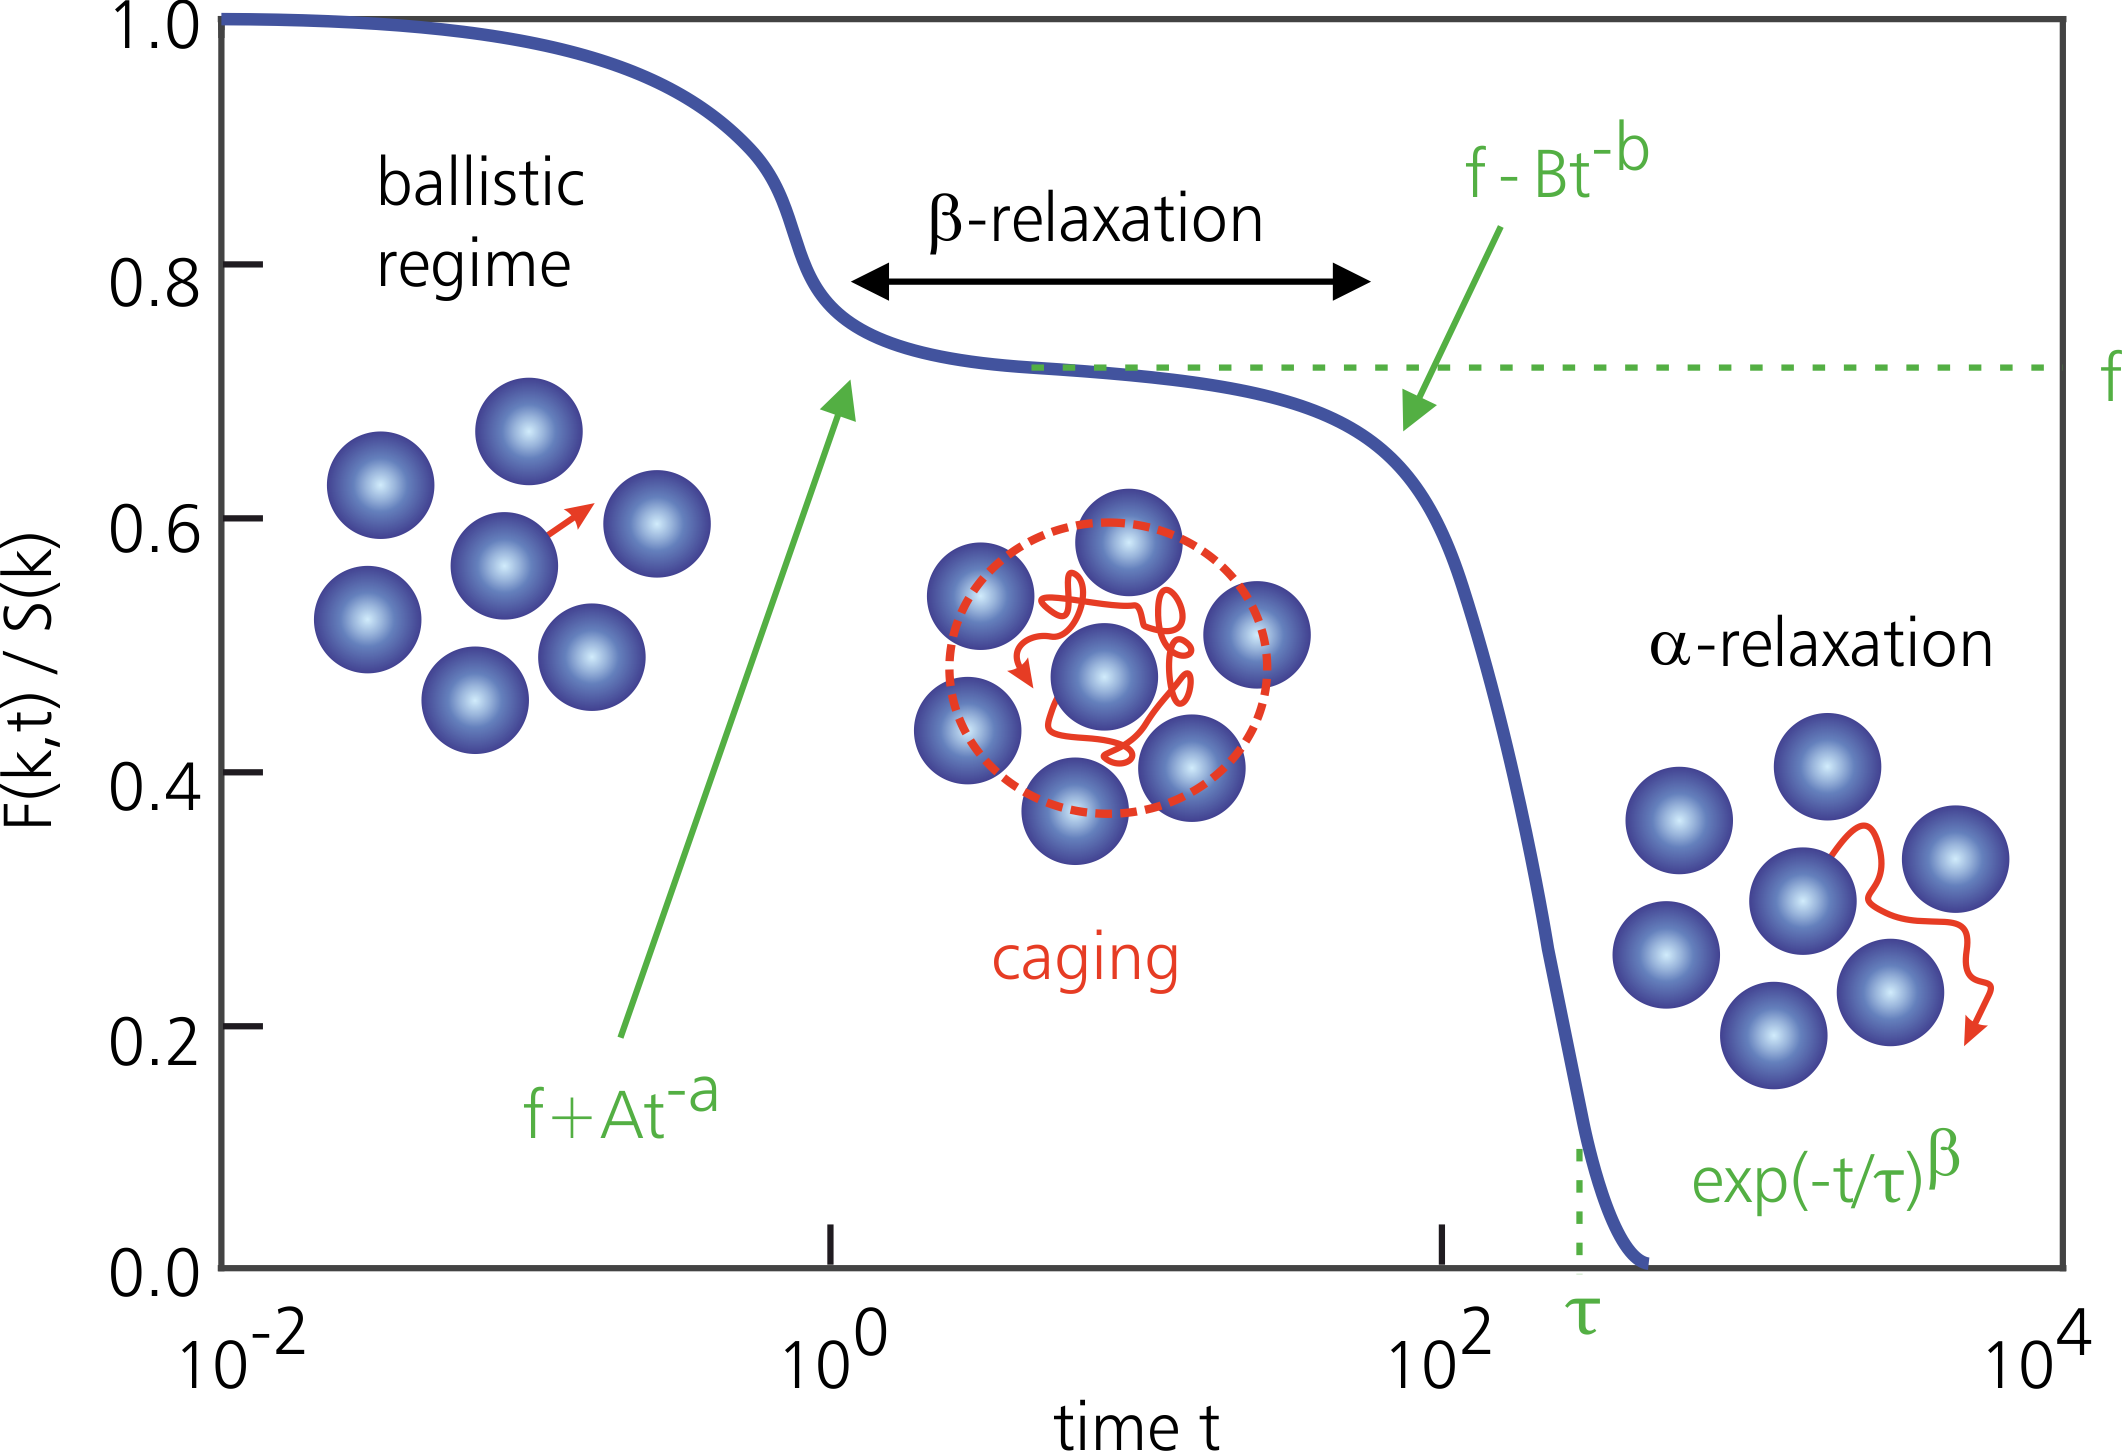
\includegraphics[width=0.9\linewidth,outer]{isf}
  \caption[Intermediate scattering function in a supercooled liquid]{
    Typical intermediate scattering function in a supercooled liquid.
    The power law predictions are from mode-coupling theory.
    Reproduced from Ref.\ \cite{JanssenFP2018}.
  }
  \label{fig:isf}
\end{SCfigure}
\todo{Remove MCT mumbo jumbo.}

A helpful framework to guide discussion of dynamical processes is \emph{transition state theory}.
In this approach a dynamical process, e.g.\ a chemical reaction, is imagined to occur through a dynamical bottleneck (Fig.\ \ref{fig:transition-state}).
We imagine evaluating a thermodynamic potential%
\marginfootnote{Which thermodynamic potential this corresponds to will depend on the ensemble.}
$\Phi$ at every point along the reaction path.
The process will then be limited by the rate of thermal fluctuations of size $\Delta \Phi$, i.e.\ those able to reach the transition state.
In equilibrium, the timescale for the process will then scale by the Boltzmann weight
\begin{equation}\label{eq:reaction-time}
  \tau \sim e^{\beta \Delta \Phi}.
\end{equation}
There will be additional kinetic prefactors out in front, however for large barriers we expect the thermodynamic contribution to dominate because of its exponential weighting.
This framework can be more rigorously justified through e.g.\ an \emph{instanton} approach \cite{LangerAP1969}.
The main limitation of transition state theory is the assumption that dynamical processes occur through effectively one-dimensional reaction paths; later, we will introduce a more sophisticated form of this framework which considers the high dimensional \emph{energy landscape}.

As an example of how useful transition state theory can be, we very briefly consider \emph{classical nucleation theory} which we will return to in more detail in chapter \ref{chapter:aerosols}.
Imagining crystallisation to occur by the spontaneous formation of the new phase inside of the liquid, then the timescale for this process will scale as
\begin{equation*}
  \tau_\mathrm{crys} \sim e^{ \beta \Delta \Phi_\mathrm{crys}}.
\end{equation*}
Then, assuming a temperature-independent barrier $\Delta \Phi_\mathrm{crys}$, the timescale for nucleation will increase exponentially as temperature is lowered allowing for the supercooled liquid to become long-lived%
\marginfootnote{Note: the time for crystallisation also scales inversely with system size, so in the thermodynamic limit nucleation occurs instantaneously unless it is strictly forbidden.}
\cite{CavagnaPR2009}.
%This is essentially the reason it is possible for supercooled liquids to exist at all, and reach an effectively time-translation invariant state without decaying to the crystal \cite{CavagnaPR2009}.
This argument is highly system dependent, as systems with small barriers to crystallisation will not be long-lived enough for the metastable liquid to be observed.
Single-component hard spheres are particularly prone to crystallise at very high densities, so polydispersity is typically introduced to frustrate the crystal structure and extend the lifetime of the supercooled liquid.
However, this process is imperfect, as even highly polydisperse systems have been found to crystallise without careful fine tuning of the size distribution \cite{BommineniPRL2019,BerthierPRL2016}.

\begin{SCfigure}
  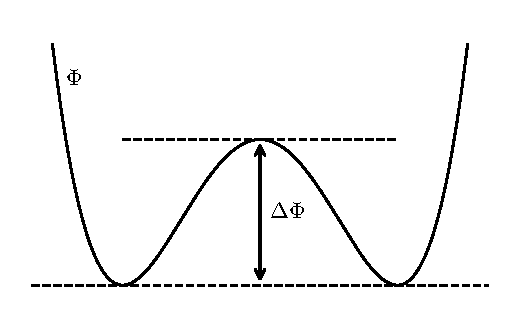
\includegraphics[width=0.7\linewidth,center]{transition-state}
  \caption[A double-well potential illustrating transition state theory]{
    A double-well potential featuring a barrier $\Delta\Phi$, representing the minimum energy required for the system to pass between the two \emph{basins}.
    The $x$-axis is the \emph{reaction coordinate}, representing a one-dimensional projection of the complete degrees of freedom.
  }
  \label{fig:transition-state}
\end{SCfigure}

Applying transition-state theory \eqref{eq:reaction-time} to relaxation time in the liquid, we may expect the $\alpha$-relaxation time to scale as
\begin{equation}\label{eq:tau-barrier}
  \tau_\alpha \sim e^{\beta \Delta \Phi_\alpha}
\end{equation}
where $\Delta \Phi_\alpha$ is the barrier to relaxation.
Naively, we might expect the barrier to remain constant with temperature, corresponding to e.g.\ the cost of breaking a bond, then we arrive at the Arrhenius law
\begin{equation}\label{eq:arrhenius-law}
  \ln{\tau_\alpha} \propto \frac{1}{T}.
\end{equation}
This argument captures the high temperature behaviour very well and, outside of soft matter, it applies reasonably well to many molecular glassformers e.g.\ silica-based materials%
\marginfootnote{That is, the material which the average person would mean when they say ``glass''.},
where relaxation essentially depends on the timescale to break a chemical bond.
Experimental data for \ce{SiO2} \cite{AngellS1995} confirms that $\ln{\tau_\alpha}$ scales linearly with $\beta$ (Fig.\ \ref{fig:angell}).
By convention, systems which scale in an Arrhenius fashion are called \emph{strong}%
\marginfootnote{This baffling naming convention has nothing to do with the mechanical properties.}
glassformers.

\begin{SCfigure}
  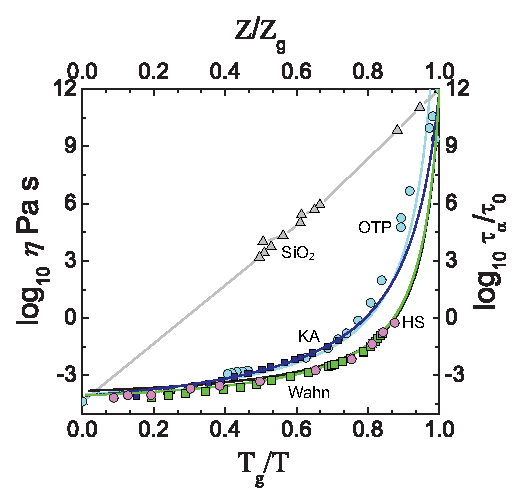
\includegraphics[width=0.9\linewidth,outer]{angell}
  \caption[The Angell plot for model systems undergoing dynamical arrest]{
    The \emph{Angell} plot \cite{AngellJNS1988} for molecular and model glassformers showing the temperature/pressure dependence of viscosity $\eta$ (or equivalently relaxation time $\tau_\alpha$).
    The molecular systems \ce{SiO2} and orthoterphenyl (OTP) respectively display the \emph{strong} and \emph{fragile} behaviours described in text, with data obtained from Refs.\ \cite{AngellS1995, BerthierPRE2009}.
    Kob-Anderson (KA) and Wahnstrom (Wahn) are binary mixtures of Lennard-Jones atoms designed to exhibit fragility.
    The compressibility $Z = \beta p / \rho$ is argued to be equivalent to inverse temperature for hard spheres (HS) \cite{BerthierPRE2009}, with data taken from Ref.\ \cite{RoyallJSM2017}.
    Reproduced from Ref.\ \cite{RoyallPR2015}.
  }
  \label{fig:angell}
\end{SCfigure}

Our focus is on soft matter, with hard spheres as the prototypical model, where the  interactions (typically van der Waals attractions) are much weaker than in molecular systems (and absent in hard spherse).
Consequently, there is less of a case for an Arrhenius relationship \eqref{eq:arrhenius-law}, and empirically we find striking deviations from it.
Many systems show \emph{super-Arrhenius} scaling with temperature (Fig.\ \ref{fig:angell}), including mixtures of Lennard-Jones atoms and molecular systems such as orthoterphenyl.
Correspondingly, systems where $\tau_\alpha$ increases more rapidly than exponential are labelled as \emph{fragile}.
A super-Arrhenius scaling of $\tau_\alpha$ implies that the thermodynamic barrier to relaxation $\Delta \Phi_\alpha$ increases with supercooling.
This means that the dynamics fundamentally changes at high densities (or low temperatures), which must be caused by the onset of \emph{collective} (or \emph{cooperative}) effects; given the weakness of bonds in soft matter, we can conclude that many particles must contribute to create a large barrier.
We will discuss this more in the next section.

Some modification is required for hard particle systems, where temperature is not a natural control parameter.
As we argued in the introduction, pressure is the only meaningful state variable.
The authors of Ref.\ \cite{BerthierPRE2009} argue that pressure plays a role equivalent to inverse temperature in athermal systems, because of similarities in their limit behaviour.
Alternatively, we could make a free volume argument, where we expect a relaxation event to involve fluctuations of volume $\Delta V$.
In equilibrium, volume fluctuations are created by reversible work $p \Delta V$ so to leading order%
\marginfootnote{The leading order behaviour can be given more justification by invoking the morphometric approach \eqref{eq:fmt-morphometric-2}, or from more general arguments which we will introduce in section \ref{sec:insertion-as-solvation}.}
we then expect
\begin{equation*}
  \tau_\alpha \sim e^{\beta p \Delta V}.
\end{equation*}
Taking $\Delta V$ as the equivalent of an energy barrier, we find the conjugate variable $\beta p$ does indeed play the role of inverse temperature.
It is usual to work with the dimensionless \emph{compressibility factor}, defined by
\begin{equation}
  Z = \frac{\beta p}{\rho},
\end{equation}
in terms of which hard spheres show the same phenomenology as thermal systems (Fig.\ \ref{fig:angell}); we find that hard spheres are comparable in fragility to various binary Lennard-Jones mixtures.
Relaxation barriers in hard spheres are entropic in nature, so perhaps it is easier to see the need for collective effects.
Moreover, the geometrical interpretation in terms of volume fluctuations $\Delta V$ provides an intuitive picture for collective motion: at high densities more particles have to move out of the way to create space for motion.

\begin{SCfigure}
  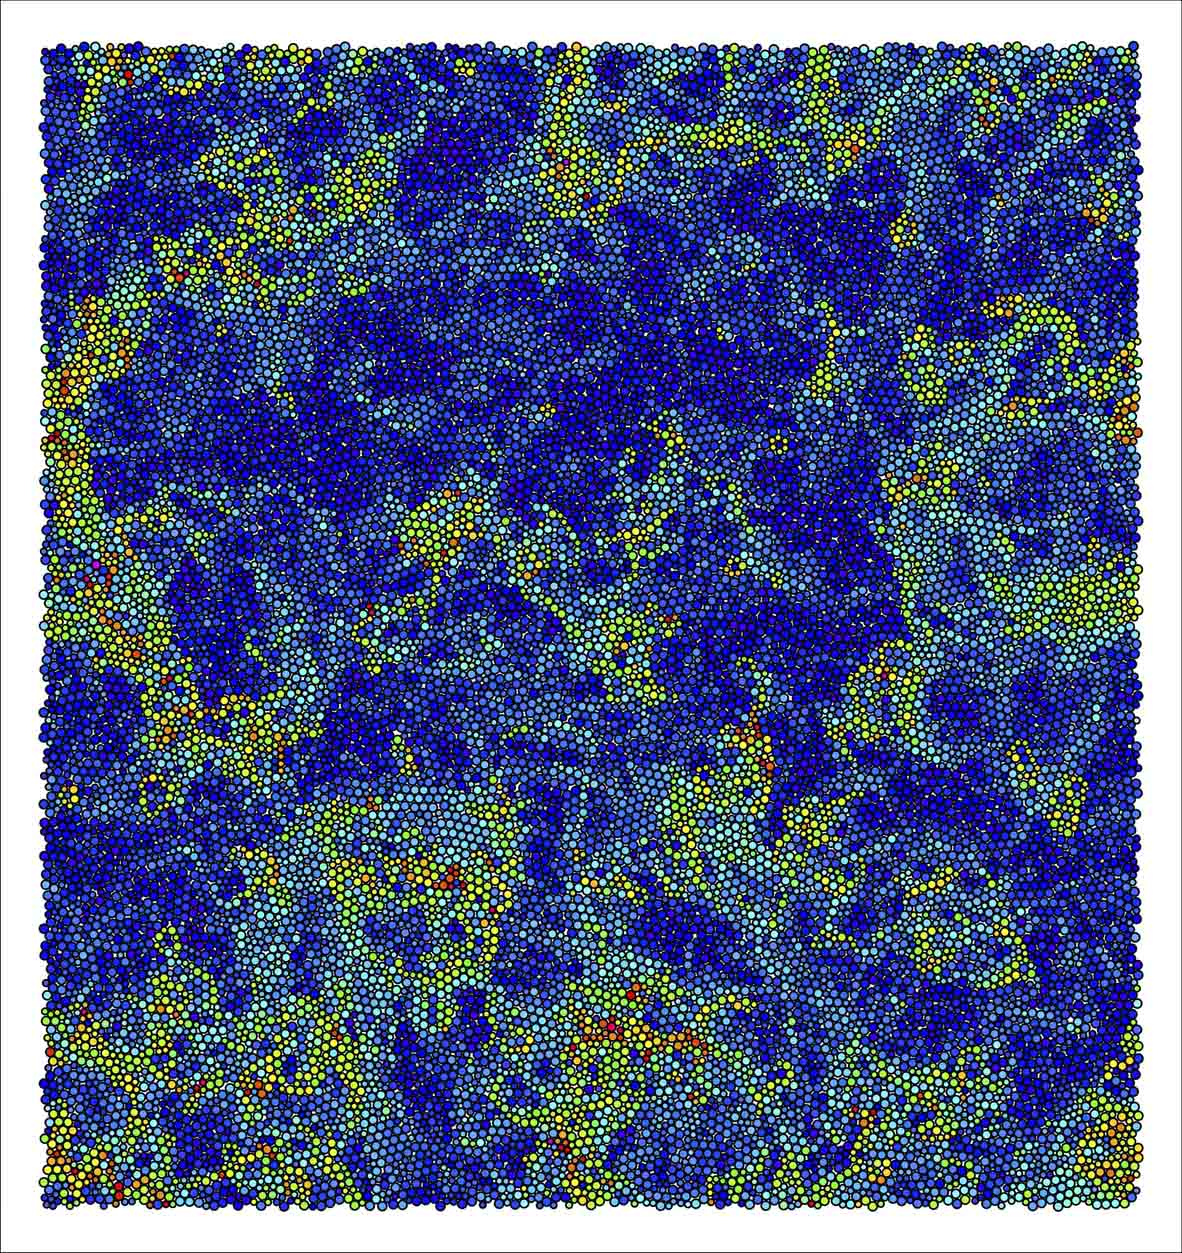
\includegraphics[width=0.7\linewidth,outer]{dynamic-heterogeneity}
  \caption[Dynamical heterogeneity in binary hard discs]{
    Dynamical heteogeneity in a binary hard disc system with a size ratio of $1:1.4$.
    Particles are coloured according to distance moved over a relaxation time $\tau_\alpha$, with blue having moved the least and red the most.
    Reproduced from Ref.\ \cite{RoyallPR2015}.
  }
  \label{fig:dynamic-heterogeneities}
\end{SCfigure}

\hl{Things I have not yet mentioned: I will do this in a single paragraph...}
\begin{itemize}
\item \hl{Operational glass transition:} $\tau_\alpha(\eta = \eta_g) = \SI{100}{\second}$
\item \hl{Dynamic heterogeneities} Fig.\ \ref{fig:dynamic-heterogeneities}
\item \hl{Stokes-Einstein breakdown}
\end{itemize}
\todo{Paragraph on facilitation vs thermodynamics (frustration, RFOT and AG)}

The main point of contention is over what causes this slow-down: whether it is driven by an underlying phase transition in the \emph{thermodynamic} view, or it is purely a kinetic effect in the \emph{dynamic} view.
These are not completely mutually exclusive viewpoints, as it is possible hybrid scenarios exist where a phase transition is 

%% We discussed the static correlation functions at length, which is fine for liquids where equilibrium occurs on a \SI{100}{\pico\second} timescale.
%% Dynamical effects are highly nontrivial at high densities.
%% As a practical definition, a glass is defined in the lab as any material for which the relaxation time exceeds \SI{100}{\second}: this point is called the experimental glass transition.
%% This is somewhat arbitrary, although the location of the glass transition point is not particularly sensitive to where you set the threshold because of how rapidly the viscosity/times are increasing around there.
%% So what do we mean by dynamical arrest.

%% Cooling a liquid.
%% Take thermodynamic quantity (e.g.\ volume, entropy, enthalpy): usually crystallise.
%% (Picture)
%% First-order transition bypassed by quick cooling.
%% Enter supercooled liquid phase.

%% Both of these conditions are violated in the glass, as this is a truly non-equilibrium state.
%% That is, we see ageing, and hysteresis in response to perturbations.
%% No longer equilibrates/relax/flows, call it a glass: occurs at glass transition.
%% Glass is a solid for all practical purposes.
%% Distinguished from glass which has dependence on preparation history, hysteresis/memory effect of heating the system (will not follow exactly the same curve until - back to the equilibrium supercooled structure), aging: averages (including correlations) evolve in time.

%% The glass transition itself is not a ``transition'' in the thermodynamic sense; there is no.
%% It's really a kind of impatience transition; the glass transition for a human would be different to the glass transition for a demigod/ent.
%% It's still a relatively robust measurement, because of the superarrhenius scaling (sc-l for pedestrians).

%% A plethora of questions related to the out-of-equilibrium properties.
%% \begin{enumerate}
%% \item Properties of out of equilibrium glass phase: very important questions for material science. Low temperature anomalies, aging behaviour, nonlinear rheology  plasticity.
%% \item Relation between glass and jamming. Jamming=zero temperature, out of equilibrium, infinite pressure.
%% \item How to avoid crystallisation.
%% \end{enumerate}

%% We will talk about this metastable branch as if it were in equilibrium.
%% \todo{create link when mention high density swap data}

%% Relationship with viscosity.
%% Flowing/not flowing is captured by viscosity: viscous slowdown same as relaxation slowdown.
%% Slightly different notion.
%% Short times $t \ll \tau$: elastic system, long times $t \gg \tau$: viscosity.
%% Time barrier is relaxation time.
%% Elasticity, viscosity in Newtonian fluids: viscoelastic behaviour (Maxwell)
%% \begin{equation}
%%   \eta = G_\infty \tau_\mathrm{relax}
%% \end{equation}
%% high frequency shear modulus is elastic property.
%% Shear modulus increases by factor 2-5 times, is dwarfed by change in relaxation time.

Having introduced the phenomenology of supercooled liquids we can now proceed to specific theories of the glass transition, beginning with an explicitly dynamical one.

\section{Mode-coupling theory}
\label{sec:mct}

The central tenet of mode-coupling theory (MCT) is to separate the liquid's degrees of freedoms into \emph{slow} and \emph{fast} variables.
Fast variables are those that thermalise very quickly, e.g.\ the solvent in a colloidal liquid, so that they can be integrated out leaving only slowly evolving variables of interest.
We advocate essentially the same philosophy, of coarse-graining onto a few dynamically relevant degrees of freedom, in developing a theory for many-body correlations in chapters \ref{chapter:morphometric-framework} and \ref{chapter:morphometric-applications}.
The difference between the two approaches is that MCT explicitly treats \emph{dynamical} processes whereas we focus on \emph{static} correlations.
We will discuss our own approach more in section \ref{sec:correlation-perspective}.

As an example of separation into fast and slow variables, consider classical Langevin equation of motion.
%, which expresses the equations of motion of a subset of the degrees of freedom.
Newton's equation for a particle in an external field becomes
\begin{equation}\label{eq:classical-langevin}
  m \ddot{\vec{r}}
  =
  \vec{\nabla} \phi_\mathrm{ext}(\vec{r})
  - \lambda \dot{\vec{r}} + \vec{f}(t)
\end{equation}
where $m$ is the particle mass, $\lambda$ is a coefficient of damping and $\vec{f}$ is the \emph{fluctuating force} from the fast variables, normally approximated as a Gaussian random field
\begin{equation*}
  \langle f_i(t) f_j(t') \rangle = 2 D \delta_{i,j} \delta(t - t'),
\end{equation*}
with diffusion constant $D$.
Here, the position $\vec{r}$ represents the slowly evolving variable of interest, whereas the remaining degrees of freedom (e.g.\ small solvent particles) are imagined to equilibrate rapidly leaving only the force field $\vec{f}$.

Mode-coupling theory starts from a formally \emph{exact} Langevin equation, which generalises the classical result \eqref{eq:classical-langevin} above.
Defining the instantaneous state of the liquid as
\begin{equation*}
  \vec{X}(t) := \begin{pmatrix} \hat\rho(\vec{r}, t) \\ \vec{\hat{j}}(\vec{r}, t) \end{pmatrix}
\end{equation*}
with instantaneous current $\vec{\hat{j}}(\vec{r}, t) := \partial \hat\rho(\vec{r}, t) / \partial t$, the generalised Langevin equation then reads \cite{ReichmanJSM2005, JanssenFP2018}
\begin{equation}\label{eq:general-langevin}
  \frac{d \vec{\widetilde{X}}(\vec{k}, t)}{dt}
  =
  i \vec{\Omega} \cdot \vec{\widetilde{X}}(\vec{k}, t)
  - \int_0^t \vec{K}(t') \cdot \vec{\widetilde{X}}(\vec{k}, t - t') \, dt'
  + \vec{f}(t)
\end{equation}
where $\vec{f}$ is (again) the fluctuating force obtained by integrating out the fast degrees of freedom, $\vec{K}(t')$ is a time-dependent \emph{memory function} containing the history of $\vec{f}$ as an autocorrelation function \cite{ReichmanJSM2005} and $\vec{\Omega}$ is the \emph{frequency matrix} containing the forces internal to the slow variables \cite{JanssenFP2018}.
Each of these terms has an allegory in the classical Langevin equation \eqref{eq:classical-langevin} above.
Similar equations to \eqref{eq:general-langevin} can be constructed for observables such as the correlation functions; the goal of MCT is to construct (and solve) an equation for $F(\vec{k}, t)$ \eqref{eq:isf} obtaining the dynamical behaviour of the liquid at long times.
The central challenge of this approach is finding suitable approximations for the memory function $\vec{K}$.
%% \begin{equation*}
%%   \vec{K}(t') = \vec{f}(0)^T \vec{f}(t') \cdot (\vec{\widetilde{X}}^T \vec{\widetilde{X}})^{-1}.
%% \end{equation*}

In the standard MCT approach, the fluctuating force is assumed to be dominated by the pair correlations so that $K$ beomes a four-point correlation function.
Then, through a second approximation where $K$ is factorised into a product of two two-point correlation functions, it is possible to construct an evolution equation for the intermediate scattering function \eqref{eq:isf} as \cite{ReichmanJSM2005}
\begin{equation}\label{eq:full-mct}
  \frac{d^2 F(k,t)}{d t^2}
  + \frac{k^2}{\beta m S^{(2)}(k)} F(k, t)
  + \int_0^t K_\mathrm{MCT}(k, t') \frac{d F(k, t - t')}{dt} \, dt'
  =
  0
\end{equation}
with
\begin{subequations}\label{eq:full-mct-coupled}
  \begin{align}
    K_\mathrm{MCT}
    &=
    \frac{\rho}{16 \pi^3 \beta m}
    \int |V_{\vec{q},\vec{k}-\vec{q}}|^2
    F(q, t) F(|\vec{k} - \vec{q}|, t)
    \, d\vec{q},
    \\
    V_{\vec{q},\vec{k}-\vec{q}}
    &=
    \frac{
      \vec{k} \cdot \vec{q} c^{(2)}(q) + \vec{k} \cdot (\vec{k} - \vec{q}) c^{(2)}(|\vec{k} - \vec{q}|)
    }{
      k
    }.
  \end{align}
\end{subequations}
The latter function $V_{\vec{q},\vec{k}-\vec{q}}$ is the so-called \emph{vertex}, which takes the pair direct correlation, and the initial condition for \eqref{eq:full-mct} is $F(k,t=0) = S^{(2)}(k)$; as such, standard MCT takes only pair correlation functions as input.
Together \eqref{eq:full-mct} and \eqref{eq:full-mct-coupled} form a non-linear coupled set of integro-differential equations that can be numerically solved, providing a reasonable description of the \emph{onset} of dynamical arrest, with deviations only becoming noticeable at deep supercooling \cite{FlennerPRE2011,BrambillaPRL2009}.

Crucially, MCT predicts a diverging timescale at $\eta \sim 0.52$ in hard spheres, where the dynamics would become completely arrested, and numerical fits to colloidal experimental data with the same power behaviour law predicted by MCT move this point up to $\eta \sim 0.58$ \cite{VanMegenPRE1994}.
However, this predicted transition must be spurious as recent experiments have managed to equilibrate colloidal hard sphere liquids up to $\eta \lesssim 0.60$ \cite{BrambillaPRL2009,HallettNC2018} and to even higher densities in simulations \cite{BerthierPRL2016}.
Despite this failing of MCT, it remains the only properly first-principles theory for treating liquid dynamics.

Extensions incorporating fluctuations can be found in Refs.\ \cite{BiroliPRL2006,SzamelPTEP2013}, and more recently a generalised MCT has been developed which avoids the uncontrolled factorisation of the pair densities \cite{JanssenPRL2015,JanssenFP2018}.
Importantly, the latter approach incorporates closures of the many-body correlation functions, which will be a central theme of later chapters; by doing this the authors were able to move the diverging timescale to higher densities, bringing the theory into better agreement with available data from simulations and experiments.

\section{Mean-field theories}
\label{sec:mean-field-glass}

We introduced MCT as an explicitly dynamical theory which attempts to model dynamical arrest in supercooled liquids by directly describing the decay of time correlation functions like $F(k, t)$.
Thermodynamics only entered implicitly into MCT through the structural input of the static structure factor $S^{(2)}(k)$.
By contast, \emph{mean-field theories} of glass take a primarily thermodynamic approach, though they are broadly compatible with the dynamical descriptions of MCT.
The mean-field picture has been rapidly gaining traction in recent years since exact solutions have been developed for hard spheres \cite{ParisiRMP2010,KurchanJSM2012,KurchanJPCB2013,CharbonneauNC2014,CharbonneauJSM2014}.
To describe mean-field theory we will invoke the concept of an \emph{energy landscape}, the natural generalisation of transition state theory introduced in section \ref{sec:glass-phenomenology} and summarised by \eqref{eq:reaction-time}.
While this conceptual framework is not unique to mean-field theories, it is most closely associated with them.

In an energy landscape description, the thermodynamic potential is interpreted \emph{geometrically} as a mapping from every point in configuration space to a `height' representing energy e.g.\ $\Phi: \mathbb{R}^{dN} \mapsto \mathbb{R}$ for an $N$ particle system.
The appeal of this approach is that physical processes can be understood \emph{topographically}: the system will spend more time at the bottom of `valleys' (minima of $\Phi$), especially at lower temperatures, and dynamics will occur primarily through low-lying `mountain passes' (saddles of $\Phi$) \cite{StillingerS1995}.
The timescales of transitions over saddles are expected to scale via the usual Boltzmann weight \eqref{eq:reaction-time}, just as in ordinary transition state theory, however this refined picture emphasises the importance of landscape \emph{connectivity}: the number, separation and relative weights of the various dynamical paths could drive the glass transition.

The energy landscape is particularly relevant in mean-field, formally corresponding to the high dimensional limit%
\marginfootnote{To understand why, consider the typical number of particle neighbours increases with dimensionality.
  Then, formally in the limit $d \to \infty$ a particle is able to achieve a macroscopic number of neighbours, equivalent to an interaction with an average field representing the rest of the system.}
$d \to \infty$, because its \emph{exact} properties can be determined.
In mean-field, hard spheres undergo a \emph{clustering} (or \emph{dynamical}) transition at a volume fraction $\eta_c$ where the landscape splits into disconnected regions \cite{ParisiRMP2010,KurchanJSM2012,KurchanJSM2016}, and the dynamics are described by an almost identical theory to MCT \cite{MaimbourgPRL2016,KurchanJSM2016}.
As configuration space becomes disconnected at $\eta_c$, the system is frozen into a single region and so the relaxation time diverges; contemporaneously, the memory function analogous to $K_\mathrm{MCT}$ in mean-field develops a plateau reflecting the fact that the density profile can no longer completely relax \cite{CharbonneauARCMP2017}.
In this light, the diverging relaxation time predicted by standard MCT is not necessarily a failure of the theory, but is indicative of this genuine mean-field transition.

Although the dynamics is singular at the dynamical transition, the thermodynamic observables are continuous as the system is compressed beyond $\eta_c$ \cite{ParisiRMP2010}.
%% Starting from the definition of the Helmholtz free energy.
%% \begin{equation*}
%%   F = \langle U \rangle - T S.
%% \end{equation*}
We can imagine what happens to the system under further compression if it could continue to sample these disconnected regions in equilibrium, i.e.\ with Boltzmann weighted measure.
The free energy, normally expressed as a sum over all microstates%
\marginfootnote{Which microstates this includes depends on the ensemble.}
$\Gamma$, can be re-expressed as a sum over a collection of \emph{mesostates} $\Gamma = \{\alpha_1, \cdots, \alpha_M\}$ giving
\begin{equation}
%\begin{subequations}
  %\begin{align}
    \Phi = \sum_{i \in \Gamma} p_i \, (\epsilon_i - k_B T \, \ln{p_i})
   % \\
    = \overline{\Phi} - T \Sigma
  %\end{align}
%\end{subequations}
\end{equation}
where $\epsilon_i$ is the energy of microstate $i$ and $p_i$ its probability measure.
In the latter step we defined%
\marginfootnote{This expression is obtained by writing the probabilty of the system being in mesostate $\alpha$ as $p_\alpha = \sum_{i \in \alpha} p_i$, then $p_i / p_\alpha$ is the probability of microstate $i$ given that the system is in this mesostate.}
\begin{subequations}
  \begin{align}
    \overline{\Phi}
    &=
    \sum_\alpha p_\alpha
    \underbrace{
      \sum_{i \in \alpha} \frac{p_i}{p_\alpha}
      \left(
      \epsilon_i - k_B T \, \ln{\frac{p_i}{p_\alpha}}
      \right)
    }_\textrm{free energy of mesostate $\alpha$},
    \\
    \Sigma &= - k_B \, \sum_\alpha p_\alpha \ln{p_\alpha}.
  \end{align}
\end{subequations}
The \emph{complexity} $\Sigma$ is an extensive quantity characterising the multiplicity of mesostates; at the dynamical transition this becomes a positive non-zero number $\Sigma(\eta = \eta_c) > 0$ corresponding to the clustering in configuration space.
As the system is compressessed further $\Sigma$ decreases \cite{KirkpatrickPRB1987,KirkpatrickPRA1989,ParisiRMP2010} corresponding to the rarefaction of clustered regions.
At a volume fraction $\eta_K > \eta_c$ an \emph{entropy crisis} occurs: $\Sigma$ vanishes, leading to the system being frozen into a single, unique region in configuration space called an \emph{ideal glass} phase \cite{KauzmannCR1948,KirkpatrickPRB1987,HallJCP1987,KirkpatrickPRA1989,ParisiRMP2010,BerthierRMP2011}.

If an equilibrium glass state in the regime $\eta \in [\eta_c, \eta_K]$ is compressed out-of-equilibrium without sampling the other clusters, a further phase transition occurs to a so-called \emph{Gardner} phase \cite{KurchanJPCB2013,CharbonneauNC2014,CharbonneauJSM2014}.
Each cluster splits further into fractal sub-regions arranged hierarchicallly.
Whereas the clustered regions formed at $\eta_c$ are geometrically dissimillar%
\marginfootnote{As measured by e.g.\ the intermediate scattering function},
these regions are close in configuration space to one another.
This phase has deep connections with the jamming transition seen at diverging pressure, providing a unified description of glass and jamming conjectured since the landmark paper of Ref.\ \cite{LiuN1998}.
Remarkably, this mean-field theory is able to predict anomalous $d$-independent critical scaling coefficients, matching those known around jamming \cite{WyartPRL2012,LernerSM2013,DeGiuliPNAS2014}.
The existence of the Gardner phase provides context for the importance of mean-field theory, but it cannot be directly connected to our approach in subsequent chapters so we will not discuss it further.
For more information on the mean-field Gardner phase see the reviews of Refs. \cite{BerthierJCP2019,CharbonneauARCMP2017}.

%% Specifically, the glass transition can be understood as the division of the energy landscape up into subunits??
%% Exact properties of the energy landscape can be determined for many mean-field systems, where it is known to play a leading role in dynamical arrest.

The mean-field picture introduces complexity as the important quantity of interest, relating the number of metastable regions in configuration space.
The relevance of mean-field descriptions in physical dimensions requires a finite-dimensional description of the supercooled liquid and its energy landscape.

%% In physical dimensions, the energy landscape does not become completely disconnected, so transitions between metastable states are possible; the dynamical transition becomes a cross-over.
%% As such, a finite-dimensional description of the supercooled liquid is needed.

%% In physical dimensions, the energy landscape does not become
%% This quantity is well-defined in mean-field because these regions are completely disconnected, however in finite dimensions transitions can always occur between them through nucleation \cite{KirkpatrickPRB1987,KirkpatrickPRA1989,BouchaudJCP2004}.
%% The dynamical transition thus becomes a cross-over, and a finite-dimensional description of the supercooled liquid is needed.

\section{Finite-dimensional theories}
\label{sec:finite-d-glass}

\begin{SCfigure}
  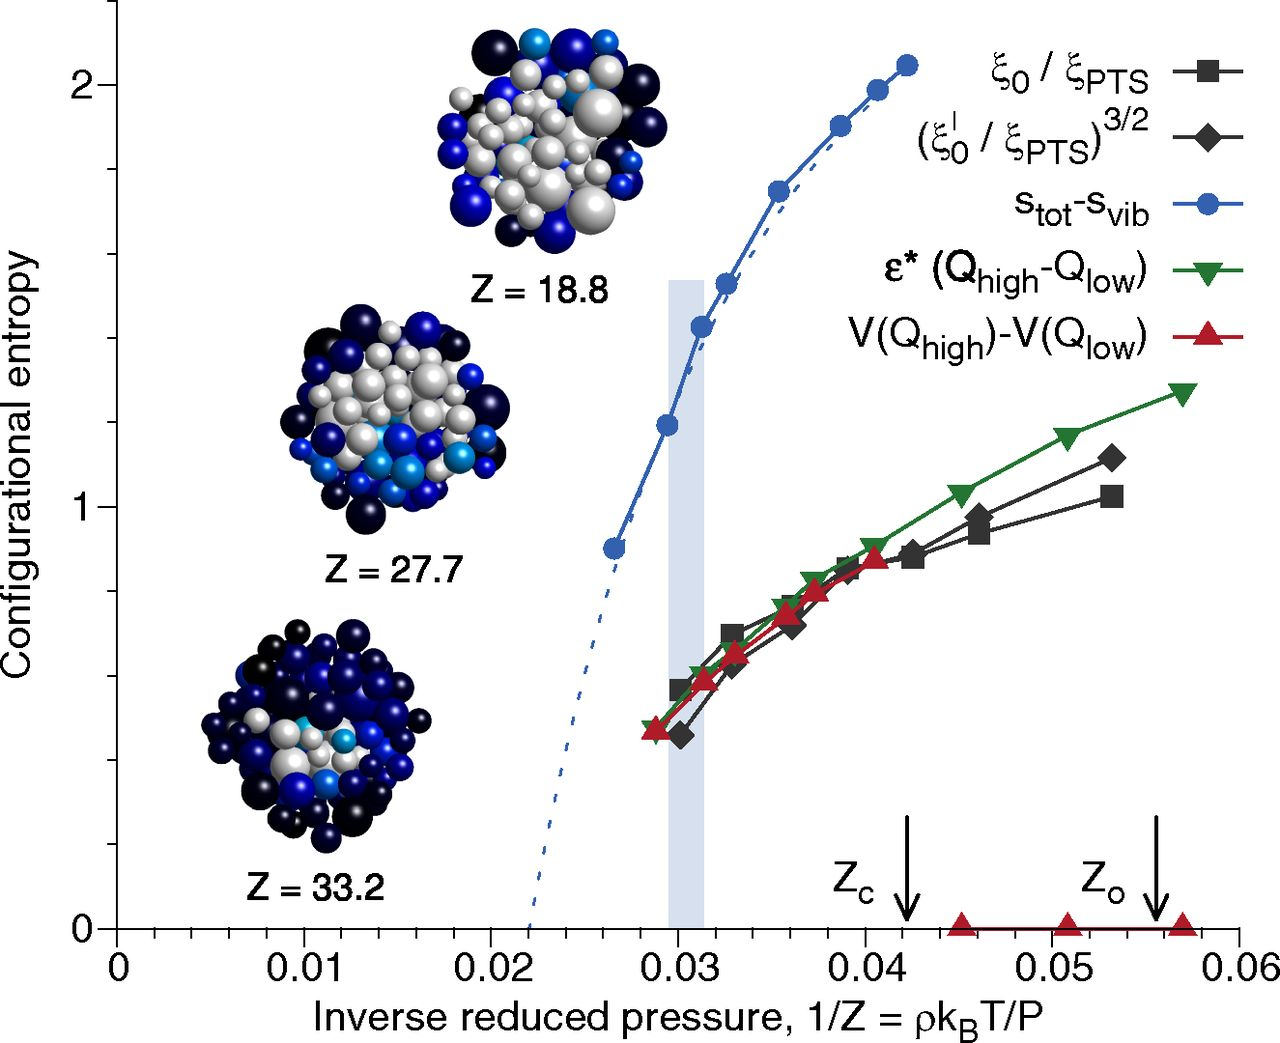
\includegraphics[width=0.9\linewidth,outer]{swap-Sconf}
  \caption[Configurational entropy in hard spheres from Monte-Carlo simulations]{
    Configurational entropy in hard spheres from novel Monte-Carlo (MC) simulations for a system with 23\% polydispersity.
    $Z_0 \approx 18$ ($\eta_0 \approx 0.56$) marks the onset pressure, above which the intermediate scattering function $F(k,t)$ decays non-exponentially, and $Z_c \approx 23.5$ ($\eta_c \approx 0.598$) is the location of the dynamical transition predicted by fitting mode-coupling theory's power-law scaling to the lower density behaviour.
    The various methods used (described in Ref.\ \cite{BerthierPNAS2017}) all broadly agree that this quantity is trending to zero at a finite pressure, suggesting the existence of a thermodynamic glass transition.
    The equation of state for this system is given in Fig.\ \ref{fig:swap-eos}.
    Reproduced from Ref.\ \cite{BerthierPNAS2017}.
  }
  \label{fig:swap-sconf}
\end{SCfigure}

%% Mean-field theories have traditionally been formulated in configuration space, in terms of the energy landscape.
%% By contast, in $d=3$ the existence of dynamical heterogeneity calls for a real space interpretation.

The relevance of mean-field ideas in physical dimensions can be seen by an interpretation of Refs.\ \cite{KirkpatrickPRB1987,HallJCP1987,KirkpatrickPRA1989}, with antecedent ideas found in \cite{KauzmannCR1948,AdamJCP1965}.
This \emph{random first-order transition} (RFOT) scenario acknowledges that the clustering of states appearing at the dynamical transition in mean-field will not be strictly metastable over finite lengthscales in finite $d$ \cite{BouchaudJCP2004,MontanariJSP2006}.
As such, the complexity is not well-defined because the metastable states will not be strictly separated with infinite barriers, though they may be arbitrarily long-lived; the dynamical transition of mean-field thus becomes a cross-over.
In finite dimensions the \emph{configurational entropy} $S_\mathrm{conf}$ is introduced as the closest equivalent to the complexity; this does not have a generally agreed upon meaning, but a common definition invokes the timescale separation between vibrational ($\beta$--) and liquid-like ($\alpha$--) dynamics.
The configurational entropy then describes the entropy of the latter process, obtained as the residual entropy after removing vibrations
\begin{equation}\label{eq:sconf}
  S_\mathrm{conf} := S - S_\mathrm{vib},
\end{equation}
though some refinement is required for polydisperse systems \cite{OzawaJCP2017,OzawaJCP2018} and where additional non-vibrational processes exist that do not relax the density profile \cite{OzawaPRL2018}.

The RFOT scenario imagines the mean-field dynamical transition as a crossover to an \emph{energy landscape dominated} dynamics.
Specifically, the number of unique (non-vibrational) states possible in a subregion of size $\xi$ will scale $\propto \exp{(s_\mathrm{conf} \xi^d / k_B)}$, where $s_\mathrm{conf} = S_\mathrm{conf} / V$ is the configurational entropy density.
A dynamical event which changes a state is expected to pay an energy penalty $\gamma_\mathrm{eff} \xi^\theta$ where $\theta \le d$ from inducing a mismatch with the surrounding fluid.
The thermodynamic potential for this subregion is then expected to adopt the form
\begin{equation}\label{eq:rfot-barrier}
  \Phi \sim \gamma_\mathrm{eff} \xi^\theta - T s_\mathrm{conf} \, \xi^d.
\end{equation}
The maximum of $\Phi$ occurs at the \emph{point-to-set}%
\marginfootnote{So-named because this lengthscale marks the crossover from the subregion being confined to a single `point' in its configuration space to a `set' of states.}
length
\begin{equation}\label{eq:rfot-xi}
  \xi_\mathrm{PS}
  := \argmax{(\Phi)}
  \sim
  \left(
  \frac{\theta \gamma_\mathrm{eff}}{d T s_\mathrm{conf}}
  \right)^\frac{1}{d-\theta},
\end{equation}
after which $\Phi$ grows infinitely negative, so the metastable states are unstable to activated dynamics for $\xi \gtrsim \xi_\mathrm{PS}$.
The RFOT interpretation thus predicts the formation of a \emph{mosaic} of droplets of typical lengthscale $\xi_\mathrm{PS}$ \cite{KirkpatrickPRB1987,HallJCP1987,KirkpatrickPRA1989,BouchaudJCP2004}.
The nature of the entropic droplets forming the mosaic state and the processes by which they relax is an active area of study \cite{BouchaudJCP2004,DzeroPRB2005,FranzJSM2005,AngeliniJSP2017,RulquinJSM2016,BiroliMeanPRB2018,BiroliFinitePRB2018}.
Notably, a lot of attention has been devoted to the treatment of the subleading term $\gamma_\mathrm{eff} \xi^\theta$.

This thermodynamic argument above concerns whether a region of the liquid \emph{will} relax eventually, but an even more direct connection with relaxation timescale was proven in Ref.\ \cite{MontanariJSP2006}.
Briefly, dynamical barriers must remain finite within a finite subregion, so they scale Arrheniusly via \eqref{eq:reaction-time}; any Arrhenius process will eventually overwhelm the super-Arrhenius scaling of $\tau_\alpha$ at deep supercooling.
Fragile behaviour then suggests a reduction in $S_\mathrm{conf}$ to limit the number of possible Arrhenius processes.
Moreover, the authors of Ref.\ \cite{MontanariJSP2006} then show that the relaxation time is rigorously bounded from above by $S_\mathrm{conf}$, proving that any diverging relaxation time \emph{must} coincide with an entropy crisis where $S_\mathrm{conf}$ becomes sub-extensive.
Measurements of the configurational entropy from simulations of hard spheres suggest a vanishing $S_\mathrm{conf}$ at finite pressure in $d=3$ (Fig.\ \ref{fig:swap-sconf}), pointing to a mean-field/RFOT scenario in hard spheres.
However, this necessarily relies on extrapolation as the point where $S_\mathrm{conf}$ vanishes cannot be reached in finite time because of the argument above.

%% Mean-field argument is thermodynamic, which in some sense is structural.
%% Structural in the sense of the energy landscape, not necessarily in real space/local structure.
%% The real space interpretation of mean-field theory is random first-order transition theory (RFOT), also called \emph{mosaic} theory.

%% In conventional condensed matter physics dynamics is determined by structure.
%% For example, crystalline solids are fixed on a lattice so do not flow, whereas liquids are disordered and are thus able to flow.
%% Soft matter systems (e.g.\ gels, foams, glasses) do not neatly fall into this paradigm: their dynamics are often arrested whilst their structure remains highly disordered.

\begin{SCfigure}
  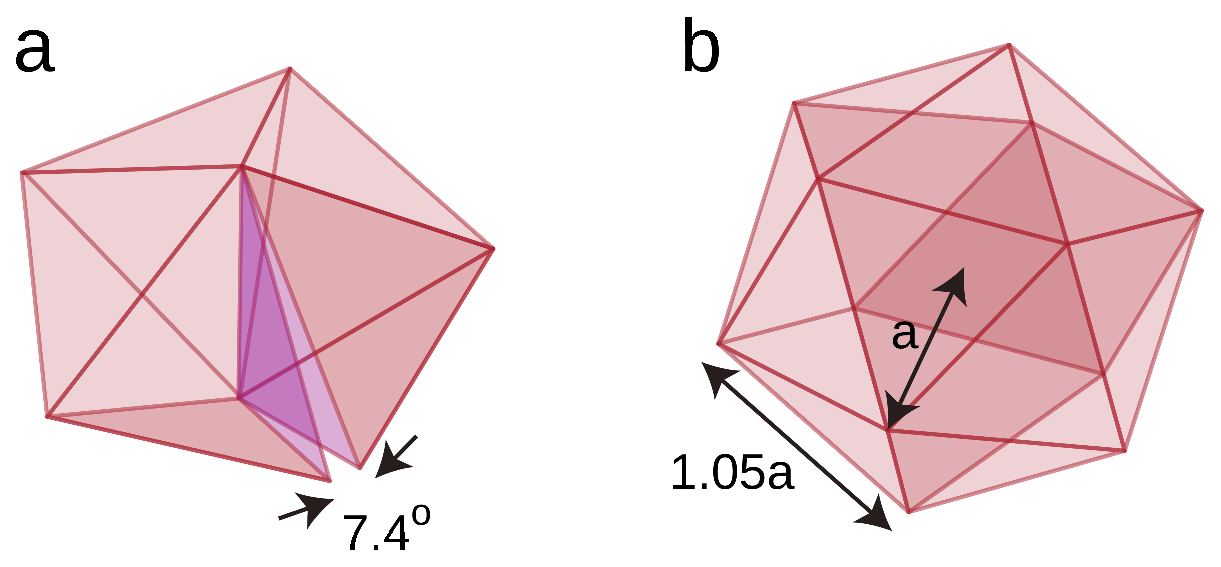
\includegraphics[width=0.7\linewidth,outer]{frustration}
  \caption[Frustration of tetrahedral structures]{
    Structures formed by combining tetrahedra.
    (a) The pentagonal bipyramid constructed from five regular tetrahedra must leave a small gap of \SI{7.4}{\degree}.
    (b) The icosahedron formed by vertices a distance $a$ from the centroid must have edge length $\sim1.05 a$, so if hard spheres of diameter $a$ were placed on the vertices they would not be in contact.
    Reproduced from Ref.\ \cite{RoyallPR2015}.
  }
  \label{fig:frustration}
\end{SCfigure}

A different scenario in physical dimensions focuses on the role of geometry.
This picture starts from the observation that crystal structures (e.g.\ the face-centred cubic introduced for hard spheres at close packing) are generally not the optimal energetic arrangement for small clusters of particles, even though they must be for bulk systems.
For example, 13 isolated Lennard-Jones atoms will preferentially arrange as vertices of a five-fold symmetric \emph{icosahedron} \cite{FrankPRS1952} (Fig.\ \ref{fig:frustration}b).
As five-fold symmetric structures cannot tesselate Euclidean space, Sir Charles Frank conjectured that glassformers suppress crystallisation through formation of icosahedra (or similar structures) \cite{FrankPRS1952}.
The above viewpoint has been developed into the more complete theory called \emph{geometric frustration} \cite{KivelsonPA1995,TarjusJPCM2005}.
This approach characterises the liquid by its \emph{locally favoured structures} (LFS), i.e.\ those structures which are energetically favoured at small length scales.
A system could have a single LFS, or a whole collection; recently, it has been shown through numerical simulations that \emph{competition} between different LFS enhances the propensity for glassformation \cite{TeichNC2019}.
Crucially, these structures do not tile space so the formation of large domains of LFS leads to the build up of \emph{frustration}, leading to a similar relation as in RFOT \eqref{eq:rfot-barrier} though the resulting phase behaviour is quite different; details can be found in the review of Ref.\ \cite{TarjusJPCM2005}.

The frustration picture is broadly compatible with the mean-field viewpoint: the propensity for a system to form certain structures can be interpretted as a manifestation (or a driving force) of a reduced $S_\mathrm{conf}$.
The downside of this scenario is that the correlation between local structure and dynamics seems to be highly system dependent \cite{HockyPRL2014}.
In hard spheres, the dominant LFS are found to be tetrahedral structures, which form very dense local packings and their presence is highly correlated with dynamics \cite{HallettNC2018} \hl{(additional citations?)}.
At high densities the tetrahedra form large connected domains \cite{HallettNC2018} rich in five-fold symmetric structures.
Spherical packings ideally form regular tetrahedra which cannot perfectly form pentagonal structures (Fig.\ \ref{fig:frustration}), so five-fold symmetric structures are highly frustrated.
A detailed review on the role of local structure in glassy systems can be found in Ref.\ \cite{RoyallPR2015}.
\todo{Should definitely cite more Royall group work here, possibly Tanaka too. What's the most appropriate cross-section of papers?}

%% The mean-field picture of glass formation interprets the dynamical slowdown entirely within a thermodynamic framework.
%% In mean-field hard spheres, formally in the limit of infinite spatial dimensions $d \to \infty$,
%% Hard spheres in mean field have been shown to have a thermodynamic glass transition, however the critical dimensions are unknown so it is unclear what happens in $d=3$. \cite{ParisiRMP2010,KurchanJSM2012,KurchanJPCB2013,CharbonneauNC2014,CharbonneauJSM2014}.
Recent numerical evidence suggests that $S_\mathrm{conf}$ only vanishes at $T=\SI{0}{\kelvin}$ for a model glassformer in $d=2$ \cite{BerthierNC2019}.
As this point cannot be crossed no thermodynamic transition can occur in $d = 2$, pointing to a lower critical dimension for mean-field theory of at least $d_L \ge 2$.
It is possible that low-dimensional fluctuations prevent any thermodynamic transition, and it has been argued that even if there is a thermodynamic transition at $\eta_K$ this may not be responsible for the dynamic slowdown seen around the operational glass transition $\eta_g \ll \eta_K$ \cite{WyartPRL2017}.
As such, there is room for alternative pictures to the mean-field/RFOT scenario.
The main opposition theory is \emph{dynamic facilitation}, which focuses on the dynamic heterogeneities as the fundamental feature of glass.
In this picture dynamical events occur through string-like motion between dynamical defects, and the relaxation time remains finite until $T = \SI{0}{\kelvin}$.
\todo{Paddy: Expand on this substantially}
For more information on dynamic facilitation we direct the reader to the review of Ref.\ \cite{ChandlerARPC2010}.
%This must trivially occur at the very least $T=0\si{K}$ where relaxation timescales diverges, however much like the lack of a phase transition in the Ising model in $d=1$ this is not a true thermodynamic phase transition because it cannot be crossed.
%So the central question of glass is what happens in $d=3$, is there a vanishing configurational entropy at a finite $T > 0$ with an accompanying thermodynamic glass transition?

%Theories concentrating on the high density glass: elastic theories.

\section{Perspective: usefulness of many-body correlations}
\label{sec:correlation-perspective}

In subsequent chapters will be heavily focusing on the treatment of static many-body correlation functions in the bulk liquid.
Here, we motivate their study for the treatment of the supercooled liquid.

Firstly, it is natural to wonder what new (thermodynamic) information is contained in the many-body correlation functions that is not already present at the pair level.
In section \ref{sec:thermodynamic-routes} we saw how the compressibility and virial routes lead to expressions of the free energy in terms of pair correlations.
This is emblematic of conventional routes to the free energy, so in some sense all of the thermodynamically relevant information is contained in the two body correlation functions.
As far as thermodynamics is concerned, we motivate their study borrowing an argument originally made by Evans \cite{EvansPrivate2019}.
The key observation is that the pair correlation yields thermodynamic quantities which are \emph{derivatives} of the free energy at an instantaneous state point, so to infer the free energy multiple state points must be sampled.
Equivalently, we could consider the derivatives of the pair correlation function.
It is straightforward to show that \cite{Santos2016}
\begin{equation}\label{eq:correlation-derivatives}
  \chi_T \rho
  \left( \frac{\partial \rho^{(n)}}{\partial \rho} \right)_{V,T}
  =
  (n - \rho V) \rho^{(n)}(\vec{r}^n)
  + \int \rho^{(n+1)}(\vec{r}^{n+1}) \, d\vec{r}_{n+1}.
\end{equation}
The important feature to take away from this expression is the presence of $\rho^{(n+1)}$; we see the emergence of higher-order correlation functions in the derivatives.
This means we could in principle measure the free energy at a single state point by introducing highly accurate measurements of the many-body correlation functions.
This is essentially the spirit of the \emph{entropy route}, which writes \cite{WallaceJCP1987}
\begin{equation}
  S = \sum_{n=1}^\infty S_n
\end{equation}
with entropic terms $S_n$ containing contributions from $n$-particle correlations.
The first few terms are given by \cite{WallaceJCP1987}
\begin{subequations}
  \begin{align}
    \frac{S_1}{V}%\langle N \rangle}
    &=
    k_B \, \rho \left( \frac{d}{2} - \ln{\rho \Lambda^d} \right),
    \\
    \frac{S_2}{V}%\langle N \rangle}
    &=
    \frac{\rho^2}{2 T}
    \int g^{(2)}(\vec{r}) \ln{g^{(2)}(\vec{r})}
    \, d\vec{r},
    \\
    \frac{S_3}{V}%\langle N \rangle}
    &=
    \frac{\rho^3}{6 T}
    %\int g^{(3)}(\vec{r}, \vec{r}') \delta w^{(3)}(\vec{r}, \vec{r}')
    \int g^{(3)}(\vec{r}, \vec{r}')
    \ln{\left(
      \frac{
        g^{(3)}(\vec{r}, \vec{r}')
      }{
        g^{(2)}(\vec{r}) g^{(2)}(\vec{r}') g^{(2)}(\vec{r} - \vec{r}')
      }
      \right)}
    \, d\vec{r} d\vec{r}'.
  \end{align}
\end{subequations}
Then, for a pair-interacting system the excess free energy is obtained as
\begin{equation*}
  \begin{split}
    \frac{\beta F^\mathrm{ex}}{V}
    =& \; \hphantom{ + } \;\,
    \frac{\rho^2}{2} \int g^{(2)}(\vec{r})
    \left( \beta u(\vec{r}) - \ln{g^{(2)}(\vec{r})} \right)
    d\vec{r}
    \\ & \;
    + \frac{\rho^3}{6}
    %\int g^{(3)}(\vec{r}, \vec{r}') \delta w^{(3)}(\vec{r}, \vec{r}')
    \int g^{(3)}(\vec{r}, \vec{r}')
    \ln{\left(
      \frac{
        g^{(3)}(\vec{r}, \vec{r}')
      }{
        g^{(2)}(\vec{r}) g^{(2)}(\vec{r}') g^{(2)}(\vec{r} - \vec{r}')
      }
      \right)}
    \, d\vec{r} d\vec{r}'
    \\ & \;
    + \mathcal{O}\left( \rho^4 g^{(4)}(\vec{r}, \vec{r}', \vec{r}'') \right),
  \end{split}
\end{equation*}
so the free energy can be directly obtained from accurate determination of the correlation functions.
%Similarly, a theory treating the many-body correlation functions must have the free energy (and phase behaviour) built in.

Secondly, while it is true that thermodynamic quantities like the pressure can certainly be inferred from the pair correlations, there is no such simple relationship for dynamic quantities.
In the absence of a thermodynamic phase transition, we would not expect the pair correlation function alone to reveal much about the nature of dynamical arrest, beyond the lack of a transition.
Even supposing the existence of a transition, the precision required to detect such a signal $g(r)$ may be arbitrarily subtle; however, any changes approaching a transition \emph{must} be magnified at the many-body level because of \eqref{eq:correlation-derivatives}.
The many-body correlation functions have potential to place the entropic droplet scenario of \eqref{eq:rfot-barrier} on more rigorous footing, by providing a means to calculate the subleading penalty term $\gamma_\mathrm{eff} \xi^\theta$.
Alternatively, the theories which postulate local mechanisms such as the LFS in geometric frustration or the dynamical defects in facilitation should be identifiable within the many-body correlation functions.

We will be focusing on many-body correlations in real space, to explore the local mechanisms proposed in theories of the glass transition described above.
In some situations the correlations in Fourier space may be more useful, most notably in MCT where many-body generalisations have already found some traction \cite{JanssenPRL2015,JanssenFP2018}.
In principle, our real space correlation functions can be Fourier transformed to obtain these, but in practice this is prohibitively expensive because of the high dimensionality of the arguments for even modest values of $n$.
However, FMT already provides an easy route to obtaining all the correlation functions in Fourier space, as described by the original papers \cite{RosenfeldPRL1989,RosenfeldJCP1990}.
We show how to obtain these below.

Fourier transforming the direct correlation functions for the uniform liquid \eqref{eq:fmt-direct-correlations-uniform-density}, and applying the convolution theorem, allows us to write the rather succinct
\begin{equation}
  \tilde{c}^{(n)}(\vec{k}^n)
  =
  - \sum_{\alpha_1, \alpha_2, \cdots, \alpha_n}
  \partial^n_{\alpha_1, \alpha_2, \cdots, \alpha_n} \beta f^\mathrm{ex} \;
  \left( \prod_{i=1}^n \widetilde{\omega}_{\alpha_i}(\vec{k}_i) \right)
  \delta(\vec{k}_1 + \vec{k}_2 + \cdots + \vec{k}_n).
\end{equation}
The delta function enforces the `ring' condition $\sum_{i=1}^n \vec{k}_i = 0$ which emerges from translational symmetry of the weight functions, reducing the dimensionality of the domain by $d$.
A further $d(d-1)/2$ degrees of freedom%
\marginfootnote{This many degrees of freedom can be removed for general $n \ge d$, but we expect fewer for $n < d$.
  For example, $n=2$ arrangements (a dimer) are isomorphic to a line so they possess $d-1$ rotational degrees of freedom.}
can be removed by exploiting rotational symmetry.
Many-particle generalisations of the static structure factor can be obtained from $\tilde{c}^{(n)}(\vec{k}^n)$ by functionally differentiating the Ornstein-Zernike equation \eqref{eq:ornstein-zernike-generic} with respect to density \cite{BarratMP1988}.

\section{Summary}

This concludes the relevant background in supercooled liquids and glasses.
In subsequent chapters we will develop a framework for treating the many-body correlation functions in real space, with the hope that it can address some of the questions outlined here.
\todo{More more more, according to Paddy. ``What does it all mean?''}

\ifdefined\includebibliography
  \newgeometry{margin=1in}
  \printbibliography
\fi

\end{document}
